

\begin{figure}[H]
    \tikzset{pics/3DBox/.style n args={3}{code={
        \tikzstyle{box}=[blue, fill=blue!20];
        \draw[box] (0, 0, 0) -- (0, #2, 0) -- (#1, #2, 0) -- (#1, 0, 0) -- cycle;
        \draw[box] (#1, 0, 0) -- (#1, 0, -#3) -- (#1, #2, -#3) -- (#1, #2, 0) -- cycle;
        \draw[box] (0, #2, 0) -- (#1, #2, 0) -- (#1, #2, -#3) -- (0, #2, -#3) -- cycle; 
    }}}

    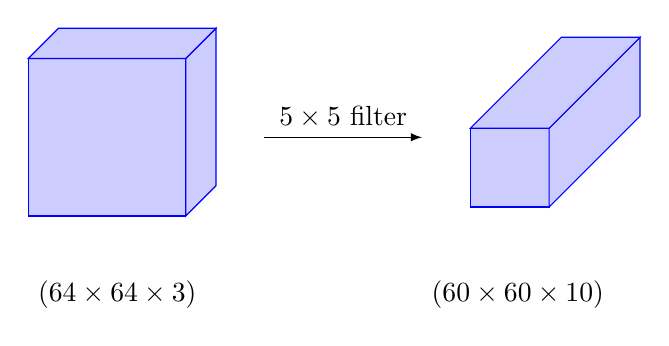
\begin{tikzpicture}
        \path pic at (0, 0, 0) {3DBox={2}{2}{1}};
        \path pic at (6, .5, 1) {3DBox={1}{1}{3}};
        \draw [-latex] (3, 1, 0) -- (5, 1, 0) node[above, midway] {$5 \times 5$ filter};

        \node [anchor=west] at (0, -1, 0) {$(64 \times 64 \times 3)$};
        \node [anchor=west] at (5 , -1, 0) {$(60 \times 60 \times 10)$};
    \end{tikzpicture}
\end{figure}

